%!TEX root = ../prace.tex

\section{Plnička kyslíkových bomb}



\begin{figure}[h!]\centering
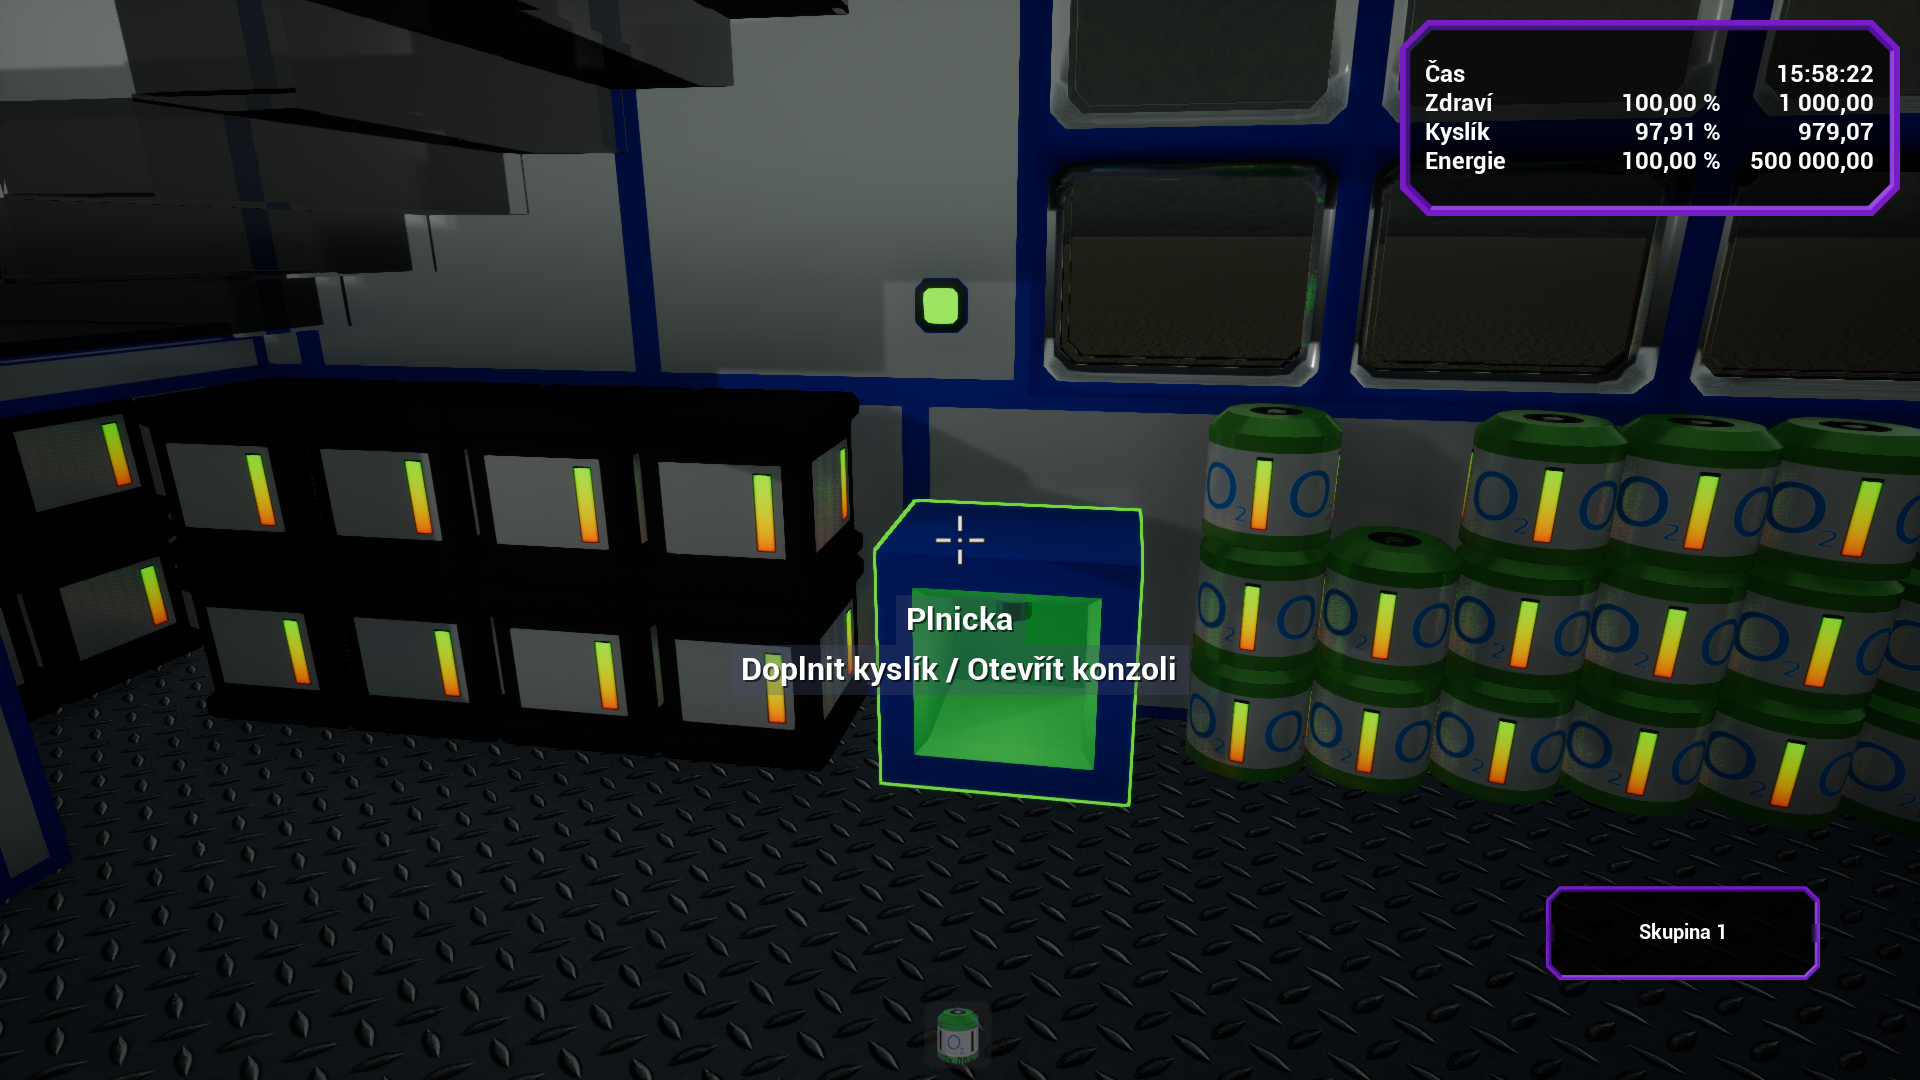
\includegraphics[ width=140mm]{../img/user/filler/0use}

\caption{Plnička kyslíkové bomby - den}
\label{fig:user_filler_0use}

\end{figure}

\begin{figure}[h!]\centering
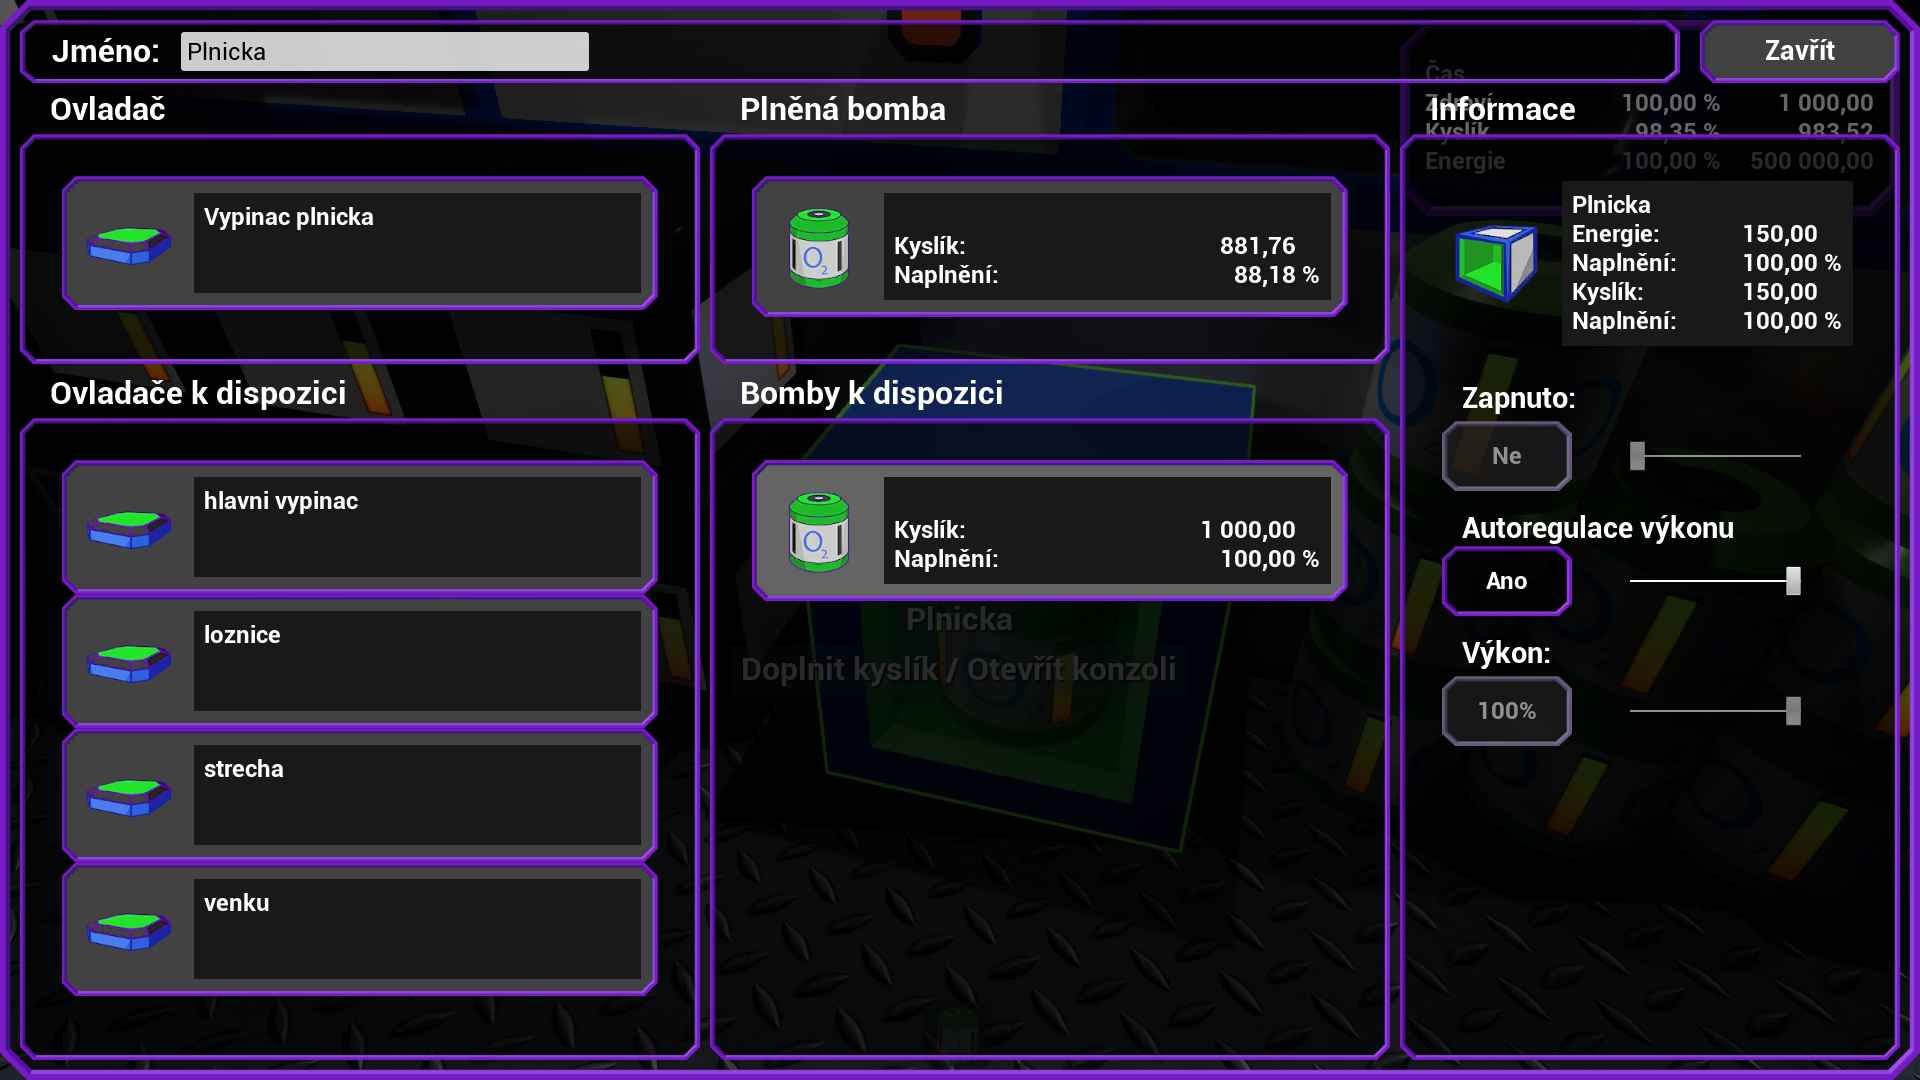
\includegraphics[ width=140mm]{../img/user/filler/1fill}

\caption{Plnička kyslíkové bomby - poledne, zataženo}
\label{fig:user_filler_1fill}

\end{figure}

\begin{figure}[h!]\centering
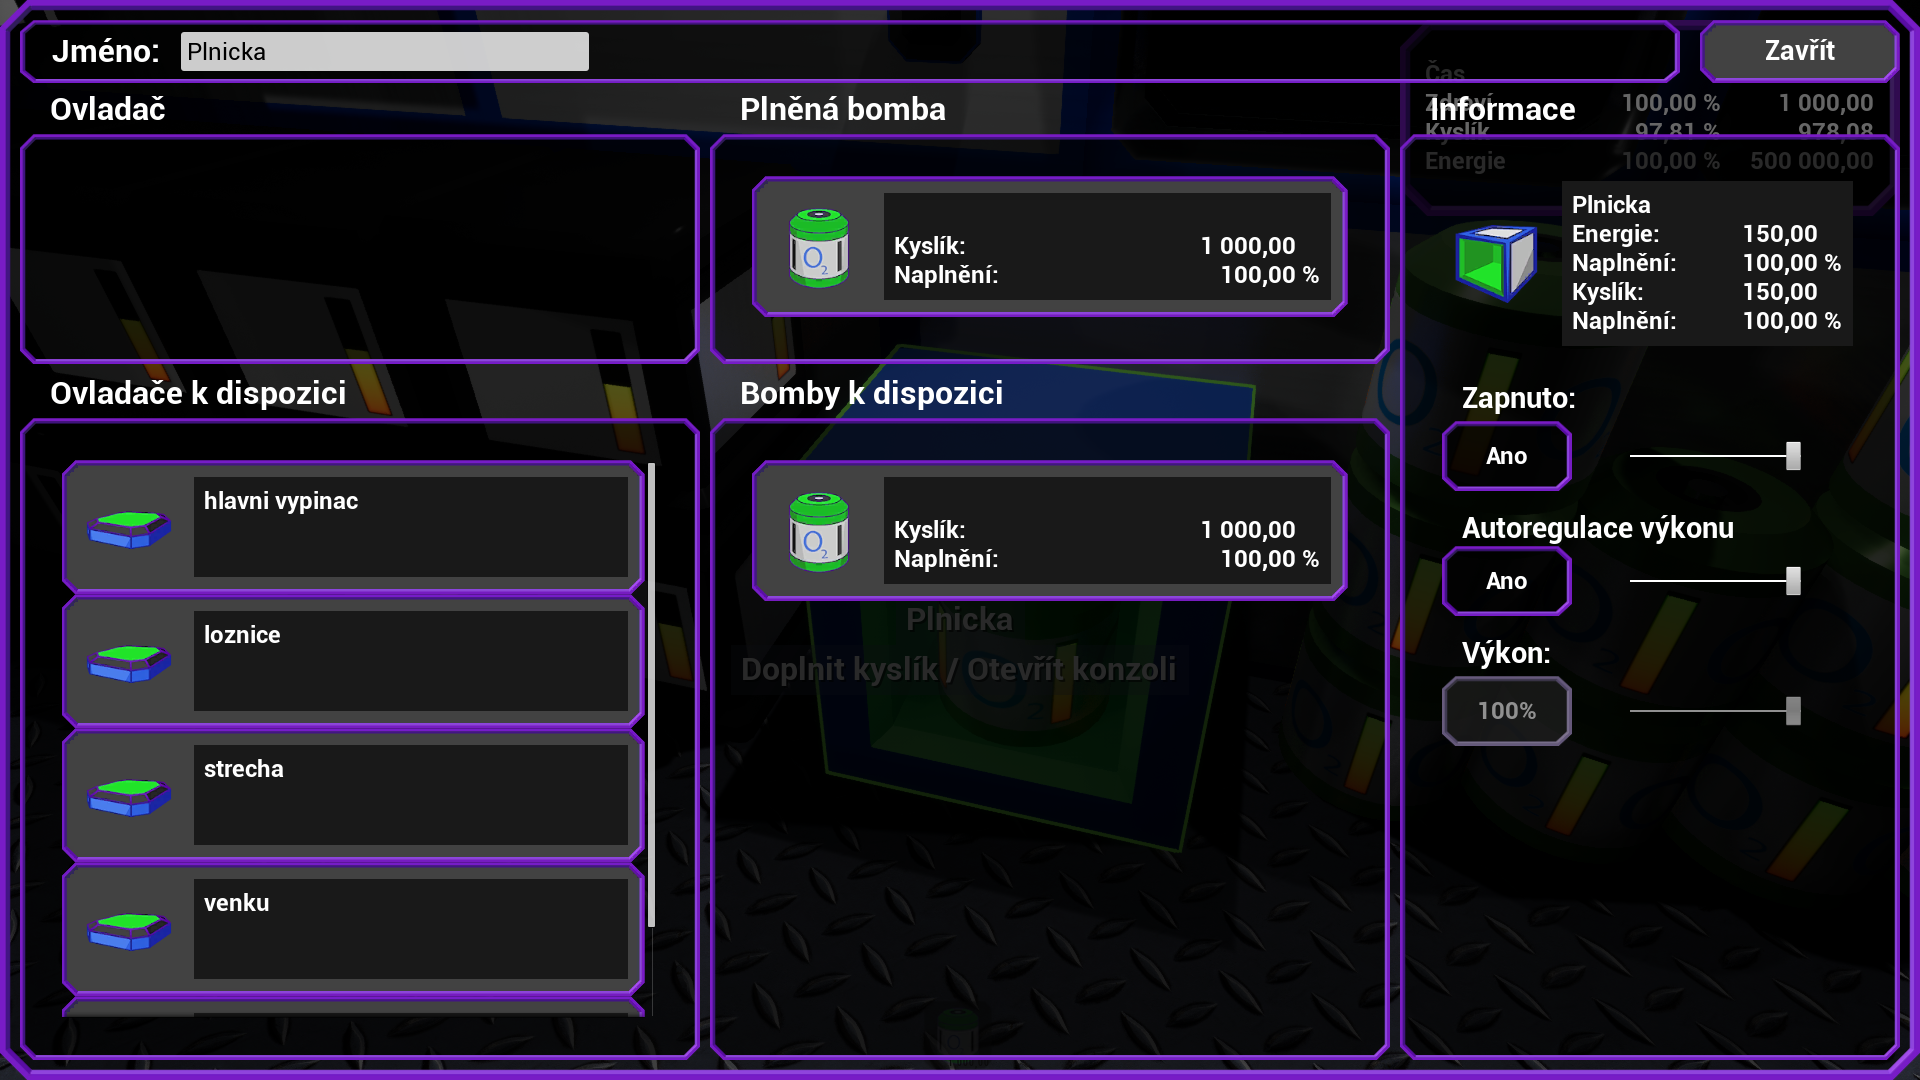
\includegraphics[ width=140mm]{../img/user/filler/2filled}

\caption{Plnička kyslíkové bomby - noc}
\label{fig:user_filler_2filled}

\end{figure}

